\documentclass[12pt]{report}
\usepackage [left=25.4mm,top=25.4mm]{geometry}
\usepackage{amsmath}
\usepackage{amssymb}
\usepackage{graphicx}
\usepackage{apacite}
\usepackage{url}
\usepackage{subfig}
\usepackage{csvsimple}
\usepackage{float}
\usepackage{tikz}


\begin{document}
\begin{titlepage}
\title{Pseudocode for MRPC Update}
\author{ Jarred M. Kvamme \\ University of Idaho \\ Department of Statistical Science }
\maketitle
\end{titlepage}

\newcommand{\indep}{\perp \!\!\! \perp}



\subsection*{1.1 - The Trio Specific Case:}

In a network consisting of three nodes: $G(V_1, T_1, T_2)$ we can identify the 5 possible topologies laid out under MRPC using results of the coefficient tests from the pair of regressions on each non-instrumental variable (Please refer to the \textbf{Appendix} at the end for Tables, Figures, and mathematical definitions).\\


\noindent \textbf{Step 1.} Preform two regressions treating each non-instumental variable as the response once:  
\begin{eqnarray}
T_1 = \beta_0 +\beta_{11}V_1+\beta_{21}T_2+{\bf \Gamma U}+ \epsilon \\
\nonumber\\
T_2 = \beta_0 +\beta_{12}V_1+\beta_{22}T_1+{\bf \Gamma U}+ \epsilon 
\end{eqnarray}


\noindent \textbf{Step 2.} calculate the correlations between the instrumental variable and $T_1$ and $T_2$, and then preform hypothesis testing on $r_{V_1,T_2}$ and $r_{V_1, T_1}$ i.e infer the marginal relationships between $V_1,T_2$ and $V_1, T_1$ \\


\noindent \textbf{Step 3.} Calculate the frequency of the minor allele of the variant/instrumental variable as $f_{\text{minor}}$. \\

\begin{quote}
\textbf{Step 3.1} - If the minor variant frequency $f_{\text{minor}}$ (allele frequency or copy number variation) from \textbf{Step 1.} is less than the predetermined threshold $\gamma$, preform the permuted regressions described in \textbf{Section 1.2} else proceed to \textbf{Step 4}
\end{quote}

\noindent \textbf{Step 4.} following \textbf{Steps 1 - 3} obtain the vector of $p$-values for hypothesis tests on $\beta_{11}, \beta_{21}, \beta_{12}, \beta_{22}, r_{V_1,T_2}$, and $r_{V_1, T_1}$ (in this order and using the nominal pvalues if $f_{\text{minor}} <\gamma$) as the vector $\bf {p}$\\

\begin{quote}
\textbf{Step 4.1} Convert the vector of $p$-values $\bf {p}$ into the indicator vector ${\bf x}_p$ where $1$ denotes a significant $p$-value at threshold $\alpha$ and $0$ denotes a nonsignificant $p$-value \\
\end{quote}

\noindent\textbf{Step 5.} - Compare ${\bf x}_p$ with the expected results for each model topology given in \textbf{Tables 1 and 2} in the \textbf{Appendix} and allocate the trio to model type for which it matches (note that models M0, M1, and M2 have two cases each depending on the directions of the edges). If no match is available allocate the trio the class "other". \\

\noindent\textbf{Step 6.} - Return the correct adjacency matrix from the inferred model type in \textbf{Step 5}


%%%%%%%%%%%%%
\subsection*{1.2 - Permuted Regression for Rare Variants} - We will apply the permuted regression described by Yang et al., 2017 whenever the instrumental variable contains a rare count at frequency $< \gamma$. The permuted regression is preformed to obtain a robust estimate of the mediation effect between the nodes $T_i$ and $T_j$ in $G(V_k, T_i, T_j)$ which may be masked in the standard regression when $V_k$ contains few observations for the minor variant. The algorithm for preforming the permuted regression is as follows:\\

\noindent \textbf{Step 1.} - permute $T_2$ in $\bf (1)$ within the levels of $V_1$ denoted $T_2^{\ast}$. Similarly, permute $T_1$ in $\bf (2)$ within the levels of $V_1$ denoted $T_1^{\ast}$.
 
\begin{quote}
\textbf{Step 1.1} - Next preform the regressions in \textbf{Section 1.1} using the permuted variables:
\begin{eqnarray}
T_1 = \beta_0 +\beta_{11}V_1+\beta_{21}^{\ast}T_2^{\ast}+{\bf \Gamma U}+ \epsilon \\
\nonumber\\
T_2 = \beta_0 +\beta_{12}V_1+\beta_{22}^{\ast}T_1^{\ast}+{\bf \Gamma U}+ \epsilon 
\end{eqnarray}
\end{quote}

\begin{quote}
\textbf{Step 1.2} - store the observed $t$-statistic for $\beta_{21}^{\ast}$ in the vector ${\bf \Theta}_{21}$ and the $t$-statistic for $\beta_{22}^{\ast}$ in the vector ${\bf \Theta}_{22}$
\end{quote}

\noindent \textbf{Step 2.} repeat \textbf{Steps 1 - 1.2} $m$ times to obtain the $m \times 1$ vectors of observed $t$-statistics ${\bf \Theta}_{21}$ and ${\bf \Theta}_{22}$. \\

\begin{quote}
\textbf{Step 2.1} - Using ${\bf \Theta}_{21}$, ${\bf \Theta}_{22}$, $t_{\text{obs}_{21}}$, and $t_{\text{obs}_{21}}$, calculate the permutation nominal p-values for $\beta_{21}$ and $\beta_{22}$ (which we will denote  respectively)
\end{quote}

\noindent \textbf{Step 3.} - retain $p_{\beta_{21}}^{\ast}$ and $p_{\beta_{22}}^{\ast}$ and return to \textbf{Step 4} in \textbf{Section 1.1} \\


%%%%%%%%%%%%%
\subsection*{1.3 - Inferring Trios Without Variants} 
We can infer the graph skeleton for any 3-node network $G(T_i, T_j, T_k)$ and uniquely infer the graph for M2. The algorithm for this is as follows:\\

\noindent \textbf{Step 1.} - Preform the regressions in \textbf{Section 1.1, Step 2} replacing the instrumental variable $V_1$ in the regressions with $T_3$  (skipping \textbf{Step 2.2} ).\\

\noindent\textbf{Step 2.} - Preform \textbf{ Section 1.1 Steps 3-4.1}\\

\noindent\textbf{Step 3.} - Compare ${\bf I}_p$ with the expected results for M2 given in \textbf{Tables 1 and 2} in the \textbf{Appendix}. \\

\noindent\textbf{Step 4.} - If ${\bf I}_p$ matches the expectation for M2, return the correct adjacency matrix for M2.\\


%----------------------------------------------------------------------------------------------------------------------
\section*{2. General Algorithm}

\textbf{Step 1.} - Given a data matrix ${\bf X}$ of $q$ instrumental variables, $p$ non-instrumental variables, and $g$ confounders. Calculate the partial correlation matrix $\bf H$ and extract the first $\lambda = \{1 : p+q\}$ rows and columns of ${\bf H}$ which represents the partial correlations between all nodes in the graph $G(V_1, V_2,...V_q, T_1, T_2, ... T_p)$.

\begin{quote}
\textbf{Step 1.1} - preform a partial correlation test on all non-diagonal entries in ${\bf H}[\lambda, \lambda]$ to obtain the $(p+q \times p+q)$ matrix of $p$-values ${\bf P}$ corresponding to the nodes in  $G(V_1, V_2,...V_q, T_1, T_2, ... T_p)$. 
\end{quote}

\begin{quote}
\textbf{Step 1.2} -For each non-diagonal entry in $\bf P$ replace significant $p$-values at threshold $\alpha$ with $1$ and nonsignificant $p$-values with $0$ to obtain the $(p+q \times p+q)$ adjacency matrix $\bf A$ for the skeleton of $G(V_1, V_2,...V_q, T_1, T_2, ... T_p)$
\end{quote}

\noindent \textbf{Step 2.} - Check all $q\times {p\choose 2}$ possible 3-node networks involving the instrumental variable(s). If the $3 \times 3$ adjacency  ${\bf A}[ijk,ijk]$ that represents the skeleton of $G(V_k, T_i, T_j)$ contains at least one edges, preallocate the trio into a list where each entry in the list is the $(n \times 3+g)$ data matrix $[V_k, T_i, T_j, {\bf U}]$ 

\begin{quote}
\textbf{Step 2.1} - Similarly, check all ${p\choose 3}$ possible 3-node networks involving only T-nodes. If the $3 \times 3$ adjacency matrix ${\bf A}[ijk,ijk]$ that represents the skeleton of $G(T_i, T_j, T_k)$ contains at least two edges, preallocate the trio into a list where each entry in the list is the $(n \times 3+g)$ data matrix $[T_i, T_j, T_k, {\bf U}]$
\end{quote}

\noindent \textbf{Step 3.} - Determine the directed structure of all trios with an instrumental variable from the list in \textbf{Step 2} using the regressions and tests outlined in \textbf{Sections 1.1-1.2}. \\


\begin{quote}
\textbf{Step 3.1} - Update the correct entries in the adjacency matrix $\bf A$ with the results for each trio in \textbf{Step 3} 
\end{quote}

\noindent \textbf{Step 4.} - For all T-node trios in \textbf{Step 2.1} obtain the $3 \times 3$ adjacency matrix from ${\bf A}[ijk,ijk]$ that represents each T-node trio.

\begin{quote}
\noindent \textbf{Step 4.1} - If ${\bf A}[ijk,ijk]$ contains a directed edge after it has been updated by \textbf{Step 3.1}, replace the instrumental variable in \textbf{Section 1.1, Step 1} with the parent node and infer the graph using regressions and tests outlined in \textbf{Sections 1.1-1.2}. 
\end{quote}

\begin{quote}
\noindent\textbf{Step 4.2} - If ${\bf A}[ijk,ijk]$ has only undirected edges after updating in \textbf{Step 3.1} replace $V_1$ in \textbf{Section 1.1, Step 1} with one of the T-nodes and infer the network using the regressions and test from \textbf{Section 1.1}\\
\end{quote} 

\noindent \textbf{Step 5.} - Use the results from \textbf{Step 4} to update the appropriate entries in adjacency matrix $\bf{A}$

\section*{3. Simulation Strategy to Validate Section 1.1}

To verify that the indicator vectors ${\bf x}_p$ derived from the the hypothesis tests in \textbf{Section 1.1} are sufficient in identifying the proposed model structures from MRPC given in \textbf{Tables 1 and 2}, we propose the following simulation methodology: \\
\\

\noindent \textbf{(1.)} - Using the linear models for the 5 basic topologies described by Badsha and Fu 2019, we propose to simulate each trio topology under varying signal strengths (and possibly sample size) using the simulation functions in the $R$ package $MRPC$.\\
\\
\noindent \textbf{(2.)}  - we then apply the algorithm proposed in \textbf{Section 1.1} to determine if the expected results given in \textbf{ Tables 1 and 2} are identified. we compare the indicator vector ${\bf x}_p$ to the expected indicator vectors for each topology and allocate the trio to one of the 5 topologies as laid out in \textbf{Section 1.1 Step 5}. Our goal is to determine if the inference for each trio is adequate for identifying the generating model or if unexpected indicator vectors arise. \\
\\
\textbf{(3.)} - Investigate, if any, the indicator vectors allocated to the "Other" class. 





\newpage
\section*{Appendix}
\begin{quote}
\textbf{Definitions}\\
$V_i$ - The $i^{th}$ instrumental variable when $q > 1$\\
$T_i$ - a non-instrumental variable/node\\
$p$ - the number of non-instrumental variables/nodes in a network\\
$q$ - the number of instrumental variables\\
$g$ - the number of confounding variables selected for a network\\
$m$ - the number of permutations to preform in a permuted regression (mediation test)\\
$n$ - the sample size of the data\\
$\bf U$ - the $(n \times g)$ matrix whose columns represent confounding variables\\
$\bf X$ - the $(n \times p+q+g)$ data matrix of all variables/nodes and all confounders\\
$\bf H$ - the $(p+q+g \times p+q+g)$ precision matrix \\
$A$ - a $(p+q \times p+q)$ adjacency matrix for the network  \\
$G(A,B,C)$ - a graph with nodes A, B, and C\\
$F(\cdot)$ - the Fisher transformation function\\
$f_{\text{minor}}$ - The frequency of the minor variant of $V_i$ (when $V$ represents a type of genetic variation)\\
$\gamma$ - the threshold frequency of the minor variant for which we determine if a permuted regression is needed\\
$\rho_{\bf x_i,x_j\cdot x_{ -(i,j)}  }$ - the partial correlation between the $i^{th}$ and $j^{th}$ columns/variables of ${\bf X}$
\end{quote}

\begin{table}[H]
\centering
\caption{- Expected results for the tests on the regression coefficients under each model scenario (trios with variants only).}
\begin{tabular}{|c||cccc|c|c|}
\hline
\bf Model  & $\bf\beta_{11}$  &  $\bf\beta_{21}$   & $\bf\beta_{12}$    & $\bf\beta_{22}$    & $ V_1 \indep T_2$    & $V_1 \indep T_1$    \\ \hline \hline
\bf M0      &  $\neq 0$            & $= 0$                  & $=0$                    & $=0$                    & Yes                          &           \\ \hline 
               &  $= 0$                 & $= 0$                  & $\neq 0$                & $= 0$                  &                                & Yes           \\ \hline
\bf M1      &  $\neq 0$            &  $\neq 0$             & $= 0$                    & $\neq 0$              & No                            &            \\ \hline
               &  $ = 0$                &  $\neq0$              & $\neq0$                & $\neq 0$              &                                & No       \\ \hline
\bf M2      &   $\neq0$            &  $\neq 0$             & $\neq0$                & $\neq0$               & Yes                          &           \\ \hline
               &   $\neq0$            &  $\neq 0$             & $\neq0$                & $\neq0$               &                                & Yes          \\ \hline
\bf M3      &   $\neq 0$           &  $= 0$                 & $\neq0$                & $=0$                   & No                           &            \\ \hline
\bf M4      &   $\neq0$            &  $\neq 0$             & $\neq0$                & $\neq0$               & No                          &             \\ \hline \hline
\bf Conditionally:  $Y \sim$& $V_i|T_j,{\bf U}$  &  $T_j|V_i, {\bf U}$   & $V_i| T_i, {\bf U}$    & $T_j|V_i,{\bf U}$    &            \\ \hline 
\end{tabular}
\end{table}

\begin{eqnarray}
T_1 = \beta_0 +\beta_{11}V_1+\beta_{21}T_2+{\bf \Gamma U}+ \epsilon \\
\nonumber\\
T_2 = \beta_0 +\beta_{12}V_1+\beta_{22}T_1+{\bf \Gamma U}+ \epsilon 
\end{eqnarray}

\begin{table}[H]
\centering
\caption{- Expected indicator table for the tests on the regression coefficients under each model scenario (trios with variants only). Note that $1$ indicates a a rejection of $H_0$ and $0$ indicates a failure to reject}
\begin{tabular}{|c||c|c|c|c||c|c|}
\hline
\bf Model  & $H_0: \bf\beta_{11} = 0$  &  $H_0:\bf\beta_{21}=0$   & $H_0:\bf\beta_{12}=0$    & $H_0:\bf\beta_{22}=0$    & $ H_0: V_1 \indep T_2$    & $H_0: V_1 \indep T_1$    \\ \hline \hline
\bf M0      &  $1$            & $ 0$                  & $0$                & $0$                    & 0                      &           \\ \hline 
               &  $0$            & $ 0$                  & $1$                & $0$                    &                         &0           \\ \hline
\bf M1      &  $1$            & $1$                  & $0$                & $1$                   & 1                        &            \\ \hline
               &  $0$            & $1$                 & $1$                & $1$                    &                           &1       \\ \hline
\bf M2      &  $1$            & $1$                 & $1$                & $1$                   & 0                         &           \\ \hline
               &  $1$            & $1$                 & $1$                & $1$                   &                            & 0          \\ \hline
\bf M3      &  $1$            & $0$                 & $1$               & $0$                   & 1                         &            \\ \hline
\bf M4      &  $1$            & $1$                 & $1$               & $1$                  & 1                         &             \\ \hline \hline

\end{tabular}
\end{table}

\begin{table}[H]
\centering
\caption{- The set up for the adjacency matrix for each 3-node network denoted by the graph $G(T_i, T_j, T_k) \ \ i,j,k\in\{1:p\}; \forall i\neq j\neq k$ found using the regressions outlined in \textbf{Section 1.3}. Each entry in the table shows the null hypothesis used for testing the edge between the node in the row and node in the column. An entry with $1$ means we keep the edge between the nodes (i.e we reject $H_0$) and a $0$ means we remove the edge between the nodes (i.e we fail to reject $H_0$)}
\begin{tabular}{|c||c|c|c|}
\hline
\bf Response  & $T_i$                                                 &  $T_j$                                           & $T_k$    \\ \hline \hline
$T_i$                &  $0$                                                  & $H_0: T_i \indep T_j|T_k, {\bf U}$   & $T_i\indep T_k |T_j, {\bf U}$                    \\ \hline 
$T_j$               &  $H_0: T_j \indep T_i| T_k, {\bf U}$    &  $0$                                               & $T_j\indep T_k|T_i, {\bf U}$                 \\ \hline
$T_k$               & $H_0: T_k \indep T_i|T_j, {\bf U}$      &  $H_0: T_k \indep T_j|T_i, {\bf U}$  & $0$                \\ \hline


\end{tabular}
\end{table}

\begin{figure}[H]
\begin{center}
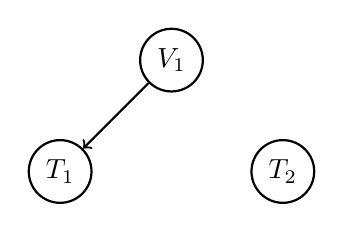
\begin{tikzpicture}[node distance={20mm}, thick, main/.style = {draw, circle}] 
\node[main] (1) {$V_1$};
\node[main] (2) [below left of=1] {$T_1$};
\node[main] (3) [below right of=1] {$T_2$} ;
\draw[->] (1) -- (2);
\end{tikzpicture}
\end{center}
\caption{M0 - $V_1\not\indep T_1 ; V_1 \indep T_2; T_1 \indep T_2$ }
\end{figure}


\begin{figure}[H]
\begin{center}
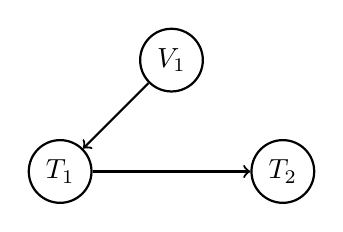
\begin{tikzpicture}[node distance={20mm}, thick, main/.style = {draw, circle}] 
\node[main] (1) {$V_1$};
\node[main] (2) [below left of=1] {$T_1$};
\node[main] (3) [below right of=1] {$T_2$} ;
\draw[->] (1) -- (2);
\draw[->] (2) -- (3);
\end{tikzpicture}
\end{center}
\caption{M1 - $V_1\not\indep T_1 ; V_1 \not\indep T_2; T_1 \not\indep T_2; V_1 \indep T_2 | T_1$}
\end{figure}

\begin{figure}[H]
\begin{center}
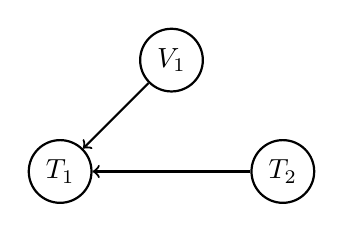
\begin{tikzpicture}[node distance={20mm}, thick, main/.style = {draw, circle}] 
\node[main] (1) {$V_1$};
\node[main] (2) [below left of=1] {$T_1$};
\node[main] (3) [below right of=1] {$T_2$} ;
\draw[->] (1) -- (2);
\draw[<-] (2) -- (3);
\end{tikzpicture}
\end{center}
\caption{M2 - $ V_1\not\indep T_1 ; V_1 \indep T_2; T_1 \not\indep T_2; V_1 \not\indep T_2 |T_1 $}
\end{figure}

\begin{figure}[H]
\begin{center}
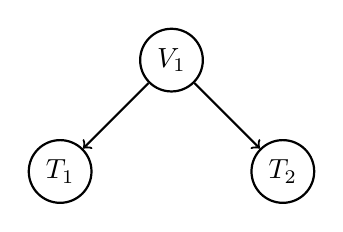
\begin{tikzpicture}[node distance={20mm}, thick, main/.style = {draw, circle}] 
\node[main] (1) {$V_1$};
\node[main] (2) [below left of=1] {$T_1$};
\node[main] (3) [below right of=1] {$T_2$} ;
\draw[->] (1) -- (2);
\draw[->] (1) -- (3);
\end{tikzpicture}
\end{center}
\caption{fig: M3 - $V_1\not\indep T_1 ; V_1 \not\indep T_2; T_1 \not\indep T_2; T_1 \indep T_2 | V_1$}
\end{figure}

\begin{figure}[H]
\begin{center}
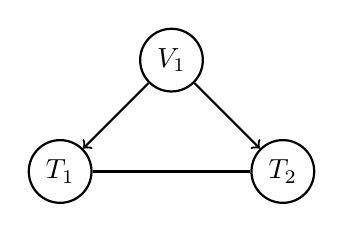
\begin{tikzpicture}[node distance={20mm}, thick, main/.style = {draw, circle}] 
\node[main] (1) {$V_1$};
\node[main] (2) [below left of=1] {$T_1$};
\node[main] (3) [below right of=1] {$T_2$} ;
\draw[->] (1) -- (2);
\draw[->] (1) -- (3);
\draw (2) -- (3);
\end{tikzpicture}
\end{center}
\caption{fig: M4 - $V_1\not\indep T_1 ; V_1 \not\indep T_2; T_1 \not\indep T_2; T_1 \not\indep T_2 | V_1$}
\end{figure}

\begin{figure}[H]
\begin{center}
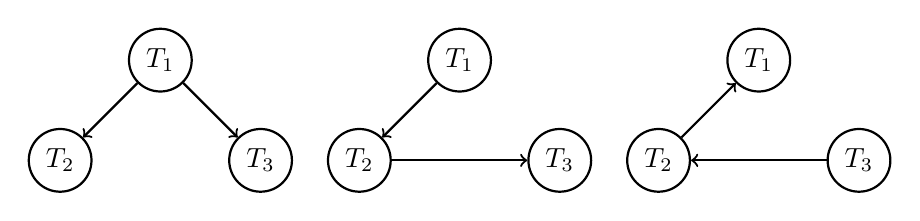
\begin{tikzpicture}[node distance={18mm}, thick, main/.style = {draw, circle}] 
\node[main] (1) {$T_1$};
\node[main] (2) [below left of=1] {$T_2$};
\node[main] (3) [below right of=1] {$T_3$} ;
\node[main] (4) [right of=1] at (2,0cm) {$T_1$};
\node[main] (5) [below left of=4] {$T_2$};
\node[main] (6) [below right of=4] {$T_3$} ;
\node[main] (7) [right of=4] at (5.8,0cm) {$T_1$};
\node[main] (8) [below left of=7] {$T_2$};
\node[main] (9) [below right of=7] {$T_3$};
\draw[->] (1) -- (2);
\draw[->] (1) -- (3);
\draw[->] (4) -- (5);
\draw[->] (5) -- (6);
\draw[->] (8) -- (7);
\draw[->] (9) -- (8);
\end{tikzpicture}
\end{center}
\caption{fig: The three graphs above are Markov equivalent meaning they share the same conditional and marginal independence relations Markove: $T_1 \indep T_3|T_2$ Minimality: $T_1 \not\indep T_2; \ T_2\not\indep T_3$ faithfulness: $T_1\not\indep T_3$ and are therefore indistinguishable from each other}
\end{figure}

\section*{Details On Statistical Methods}

\subsection*{Calculating Precision}

Given a data matrix ${\bf X}$ of $q$ instrumental variables, $p$ non-instrumental variables, and $g$ confounders:\\
Assuming $\bf X$ is centered:

\[ X \sim N_k({\bf 0}, {\bf\Sigma})  \ \ \ \text{for} \ k=p+q+g\]
 
Then the precision matrix of $\bf X$ is defined as 

\[  {\bf H} = {\bf \Sigma}^{-1} \]

$\bf H$ can be scaled to the partial correlation matrix for the entries in $\bf X$. Given the entry in the $i^{th}$ row and $j^{th}$ column of $\bf H$:

\[  {\bf x}_i, {\bf x}_j | {\bf x}_{-(i,j)} = - \frac{h_{ij}}{\sqrt{h_{ii}}\sqrt{h_{jj}}} = \hat{\rho}_{\bf x_i,x_j\cdot x_{ -(i,j)}  }\]

which is a measure of the association between the $i^{th}$ and $j^{th}$ columns/variables in $\bf X$ conditioned on all other variables. \\
\\
The Fisher transformation can be used to formulate a test for each partial correlation coefficient of interest:

\[ \frac{\sqrt{n - |{\bf x_{-i,j}}| -3}}{2}\ln\left( \frac{1+\hat{\rho}_{\bf x_i,x_j\cdot x_{ -(i,j)}  }}{1-\hat{\rho}_{\bf x_i,x_j\cdot x_{ -(i,j)}  }} \right)  \approx N(0,1)\]

where null and alternative hypotheses are 
\[ H_0:  \hat{\rho}_{\bf x_i,x_j\cdot x_{ -(i,j)}  } = 0 \ \ \ H_A: \hat{\rho}_{\bf x_i,x_j\cdot x_{ -(i,j)}  }\neq 0\]

\[  \text{reject $H_0$ if} \ \  | Z_{\text{obs}}| > Z_{1-\alpha/2 }\]

by applying the cases:

\[  a_{i,j} = \begin{cases}1 & \text{if} \ \ 2\times P(Z>|Z_{\text{obs}}|)<\alpha \\
                                      0 & \text{else} 
  \end{cases} \ \ \forall i,j \in \{1:p+q\}\]

we can obtain the $(p+q \times p+q)$ adjacency matrix $\bf A$ for the network skeleton\\

\subsection*{Permutated Regression mediation test}
 repeat $m$ times: permute $T_j$ in $\bf (1)$ within the levels of $V_i$ denoted $T_j^{\ast}$. Similarly, permute $T_i$ in $\bf (2)$ within the levels of $V_k$ denoted $T_i^{\ast}$. Next preform the regressions using the permuted variables:

\begin{eqnarray}
T_i = \beta_0 +\beta_{1i}V_k+\beta_{2i}^{\ast}T_j^{\ast}+{\bf \Gamma U}+ \epsilon \\
\nonumber\\
T_j = \beta_0 +\beta_{1j}V_k+\beta_{2j}^{\ast}T_i^{\ast}+{\bf \Gamma U}+ \epsilon \nonumber 
\end{eqnarray}

 Let ${\bf \Theta}_{2i}$ and ${\bf \Theta}_{2j}$ denote the $(m \times 1)$ vectors representing the collection of $t$ statistics from the wald tests on $\beta_{2i}^{\ast}$ and $\beta_{2j}^{\ast}$ coefficients (respectively) from the permuted regressions in \textbf{Step 2.}. such that:

\[ {\bf \Theta}_{2i} = \left[ T_{2i}^{\ast (1)}, \ T_{2i}^{\ast (2)}, \ T_{2i}^{\ast (3)}, \cdots \right] \]

\[ {\bf \Theta}_{2j} = \left[ T_{2j}^{\ast (1)}, \ T_{2j}^{\ast (2)}, \ T_{2j}^{\ast (3)}, \cdots \right]  \]

We next test the conditional association between $T_i$ and $T_j$ using the nominal test defined by Yang et. al., 2017. Let $T_{\text{obs}_{2i}}$ be the observed wald statistic from $\bf (1)$ and $T_{\text{obs}_{2j}}$ be the observed wald statistic from $\bf(2)$. We formulate the testable hypotheses: 

\[ H_0: T_{\text{obs}_{2i}} = \mu_{2i}^{\ast}, \ \ H_A: T_{\text{obs}_{2i}} \neq \mu_{2i}^{\ast} \]
and
\[ H_0: T_{\text{obs}_{2j}} = \mu_{2j}^{\ast}, \ \ H_A: T_{\text{obs}_{2j}} \neq \mu_{2j}^{\ast} \]

where $\mu_{2i}^{\ast}$ and $\mu_{2j}^{\ast}$ denote the centers of the non-central $t$-distributions of ${\bf \Theta}_{2i}$ and ${\bf \Theta}_{2j}$ respectively. Therefore the mediation test statistic is:

\[ Z_{\text{obs}_{ij}} = \frac{T_{\text{obs}_{ij}} - \frac{\sum {\bf \Theta}_{ij}}{m} }{SE({\bf \Theta}_{ij})} \]

where we 

\[ \text{reject $H_0$ if} \ \ \ 2\times P(Z >  |Z_{\text{obs}_{ij}}|) < \alpha \]

\subsection*{Inferring the Network Among Non-Instrumental Variables}

Because we infer the network among all 3-node networks involving an instrumental variable first, we have additional information for each 3-node network among T-nodes. When we lack an instrumental variable, we can only uniquely infer M2. As a result we cannot distinguish M1 and M3 due to Markov equivalence, but we are able to determine the undirected graphs of M0 and M4. (\textbf{Figure 6}). Exploiting the information provided by the associations between the T-nodes and the instrumental variable(s) we obtain in \textbf{Step 3} of the \textbf{General Algorithm} we can actually view the problem as a partially inferred network among 4 nodes i.e the graph $G(V_1, T_1, T_2, T_3)$.\\


\begin{center}
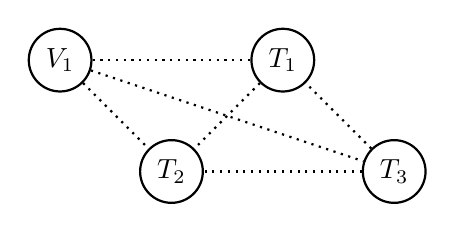
\begin{tikzpicture}[node distance={20mm}, thick, main/.style = {draw, circle}] 
\node[main] (1) {$T_1$};
\node[main] (2) [below left of=1] {$T_2$};
\node[main] (3) [below right of=1] {$T_3$};
\node[main] (4) [above left of=2]{$V_1$};
\draw[dotted] (4) -- (1);
\draw[dotted] (1) -- (2);
\draw[dotted] (4) -- (3);
\draw[dotted] (4) -- (2);
\draw[dotted] (3) -- (1);
\draw[dotted] (3) -- (2);
\end{tikzpicture}
\end{center}
The above graph demonstrates how we may view the problem of classifying trios of T-nodes, by exploiting whatever relationships exist in the subnetwork of the  graphs $G(V_1, T_1,T_2), G(V_1,T_1,T_3)$ and $G(V_1, T_2,T_3)$. 
\\


\textbf{Example 1:  v-structure in $G(T_1, T_2, T_3)$}
\\

\begin{center}
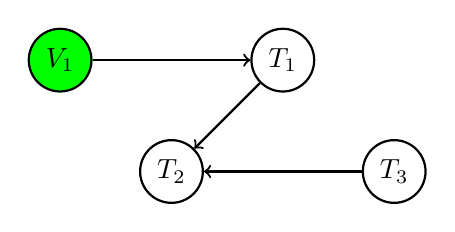
\begin{tikzpicture}[node distance={20mm}, thick, main/.style = {draw, circle}] 
\node[main] (1) {$T_1$};
\node[main] (2) [below left of=1] {$T_2$};
\node[main] (3) [below right of=1] {$T_3$};
\node[circle, draw, fill=green] (4) [above left of=2]{$V_1$};
\draw[->] (4) -- (1);
\draw[->] (1) -- (2);
\draw[->] (3) -- (2);
\end{tikzpicture}
\end{center}

Take the example above as one such network that may exist among the nodes $V_1, T_1, T_2, T_3$ defined by the individual graph types:

\[ G(V_1, T_1, T_2, T_3)=\begin{cases}G(V_1,T_1,T_2):M1 \\ G(V_1, T_1,T_3):M0 \\ G(V_1, T_2,T_3):Other \\  G(T_1,T_2,T_3):M2 \end{cases}\]

Therefore, we require the step of inferring $G(T_1, T_2, T_3)$ to identify v-structures in the non-instrumental variable network of T-nodes. If we did not preform a separate trio analysis for the nodes $T_1, T_2, T_3$ we could still infer all the edges in the above graph, however the edge between $T_2$ and $T_3$ would be left undirected. Therefore, by including this step in the algorithm we are able to direct an additional edge whenever the relationship between $T_i, T_j, T_k$ is of type M2:\\

\textbf{Example 2: No v-structure in $G(T_1, T_2, T_3)$}

\begin{center}
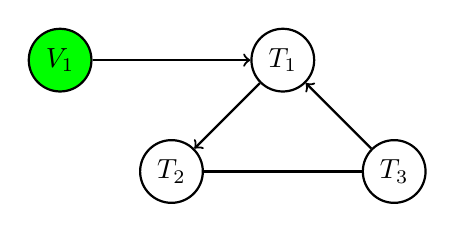
\begin{tikzpicture}[node distance={20mm}, thick, main/.style = {draw, circle}] 
\node[main] (1) {$T_1$};
\node[main] (2) [below left of=1] {$T_2$};
\node[main] (3) [below right of=1] {$T_3$};
\node[circle, draw, fill=green] (4) [above left of=2]{$V_1$};
\draw[->] (4) -- (1);
\draw[->] (1) -- (2);
\draw[->] (3) -- (1);
\draw (3) -- (2);
\end{tikzpicture}
\end{center}

\[ G(V_1, T_1, T_2, T_3)=\begin{cases}G(V_1,T_1,T_2):M1 \\ G(V_1, T_1,T_3):M2 \\ G(V_1, T_2,T_3):Other \\ G(T_1, T_2, T_3):M4 \end{cases}\]

This is a counter example where the inference for the subnetwork for $T_1, T_2, T_3$ would be returned as M4 which is undirectable in the absence of the PMR assumption. As a result the subnetworks for the combinations of nodes involving the variant fully specify the graph $G((V_1, T_1, T_2, T_3)$\\

\textbf{Example 3: Multi-instrumental Variable Network with T-node V-structure }

\begin{center}
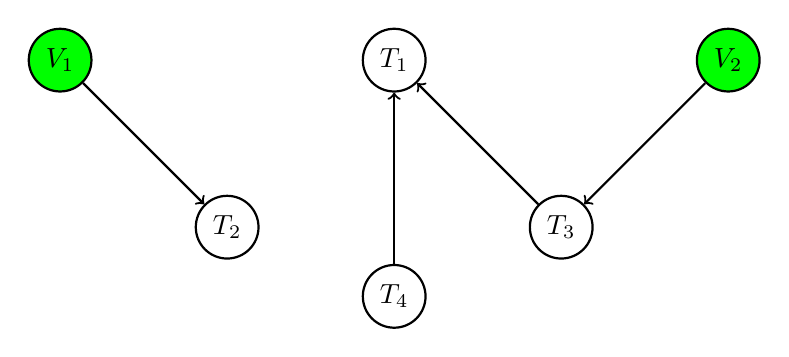
\begin{tikzpicture}[node distance={3cm}, thick, main/.style = {draw, circle}] 
\node[main] (1) {$T_1$};
\node[main] (2) [below left of=1] {$T_2$};
\node[main] (3) [below right of=1] {$T_3$};
\node[main] (4) [below of=1] {$T_4$};
\node[circle, draw, fill=green] (5) [above left of=2] {$V_1$};
\node[circle, draw, fill=green] (6) [above right of=3] {$V_2$};
\draw[->] (6) -- (3);
\draw[->] (5) -- (2);
\draw[->] (3) -- (1);
\draw[->] (4) -- (1);
\end{tikzpicture}
\end{center}

\[ G(V_1, V_2, T_1, T_2, T_3, T_4)=\begin{cases}G(V_1,T_1,T_2):M0 \\ G(V_1, T_1,T_3):Other \\ G(V_1, T_1,T_4):Other \\ 
									 G(V_1, T_2,T_3):M0 \\G(V_1, T_2,T_4):M0 \\ G(V_1, T_3,T_4):Other \\  
                                                                         G(V_2,T_1,T_2):Other \\ G(V_2, T_1,T_3):M1 \\ G(V_2, T_1,T_4):Other \\ 
									 G(V_2, T_2,T_3):M0 \\G(V_2, T_2,T_4):Other \\ G(V_2, T_3,T_4):M0 \\
                                                                        G(T_1, T_2, T_3):M0 \\ G(T_1, T_2, T_4):M0 \\ G(T_1, T_3, T_4):M2 \\
                                                                        G(T_2, T_3, T_4):Other\end{cases}\]

This is a counter example where the inference for the subnetwork for $T_1, T_2, T_3$ would be returned as M4 which is undirectable in the absence of the PMR assumption. As a result the subnetworks for the combinations of nodes involving the variant fully specify the graph $G((V_1, T_1, T_2, T_3)$
























\end{document}